\title{DINOv3}
%\subtitle{Section 2: Information Theory of Deep Learning}
\author{Oriane Siméoni et al.}
\date{\today}


{\setbeamertemplate{footline}{}
\begin{frame}[plain]
  \vspace{0.8cm}
  \titlepage
  \vfill
  {\color{Accent}\rule{2.2cm}{2pt}}
\end{frame}
}


% Background, Motivation and DINOv2
\begin{frame}{Ideas Julian Part}
\begin{itemize}
    \item Motivate importance of good feature representation for any downstream task
    \item Cover SL, WSL and SSL approaches to said goal
    \item Introduce DINOv2, it's great attention to proper data curation and results
    \item Talk about (Fan et al., 2025) and why scaling from 1B to 7B failed before DINOv3
\end{itemize}
\end{frame}

% DATA CURATION
\begin{frame}{Data Curation}
    17B public Instagram images.\\
    $\rightarrow$ DINOv2 embeddings\\
    $\rightarrow$ two routes of curation:

    \begin{itemize}
        \item \textbf{Clustering:} Hierarchical k-means + balanced sampling $\rightarrow$ LVD-1689M.
        \item \textbf{Retrieval:} Find images similar to seed datasets.
        \item \textbf{Additional datasets:} ImageNet1k, ImageNet22k, Mapillary.
    \end{itemize}

    
\end{frame}

\begin{frame}{Model Scaling / Architecture}
%\usepackage{booktabs}
\begin{itemize}
    \item Scaled mostly width, not depth.
    \item Go from learned positional embeddings to RoPE.
\end{itemize}
\begin{table}[h]
\centering
\begin{tabular}{lcc}
\hline
 & \textbf{DINOv2} & \textbf{DINOv3} \\
\hline
Parameters & 1.1B & 6.7B \\
Blocks & 40 & 40 \\
Embedding dim. & 1536 & 4096 \\
Attention heads & 24 & 32 \\
Patch size & 14 & 16 \\
Position encoding & Learned & RoPE \\
\hline
\end{tabular}
\end{table}
\end{frame}

\begin{frame}{Training at scale}

\begin{itemize}
    \item 1M iterations of initial pre-training
    \item First 100k iterations is warmup
    \begin{itemize}
        \item learning rate increases linearly to $4\times10^{-4}$
        \item teacher temperature is also warmed up linearly
    \end{itemize}
    \item After warmup:
    \begin{itemize}
        \item constant learning rate
        \item constant teacher temperature
    \end{itemize}
    \item Replaces the cosine schedules used in DINOv2
    \item Global performance improves with longer training, while dense performance degrades after about 200k iterations
    \item Gram anchoring is introduced after 1M iterations to improve dense performance
\end{itemize}
\end{frame}


%------------------------------------------
% Part 3
%------------------------------------------


%------------------------------------------
% Part 4 
%------------------------------------------
\begin{frame}{Post-training}
    \begin{enumerate}
        \item \textbf{Higher Resolution Adaptation} - Gram is essential\\
        10k additional iteration with mixed resolution sampling \\ Global crops from \{512, 768\} and local crops from \{112, 168, 224, 336\} \vspace{5px}
        \item \textbf{Model Distillation with shared teacher inference} \\
        7B frozen teacher → ViT-S, ..., H+, ConvNeXt
        \vspace{5px}
        \item \textbf{Aligning DINOv3 with Text using LiT approach} \\
        Frozen vision transformer - train text encoder contrastively on [CLS ; mean-pooled patches]
    \end{enumerate}
    \begin{figure}
        \centering
        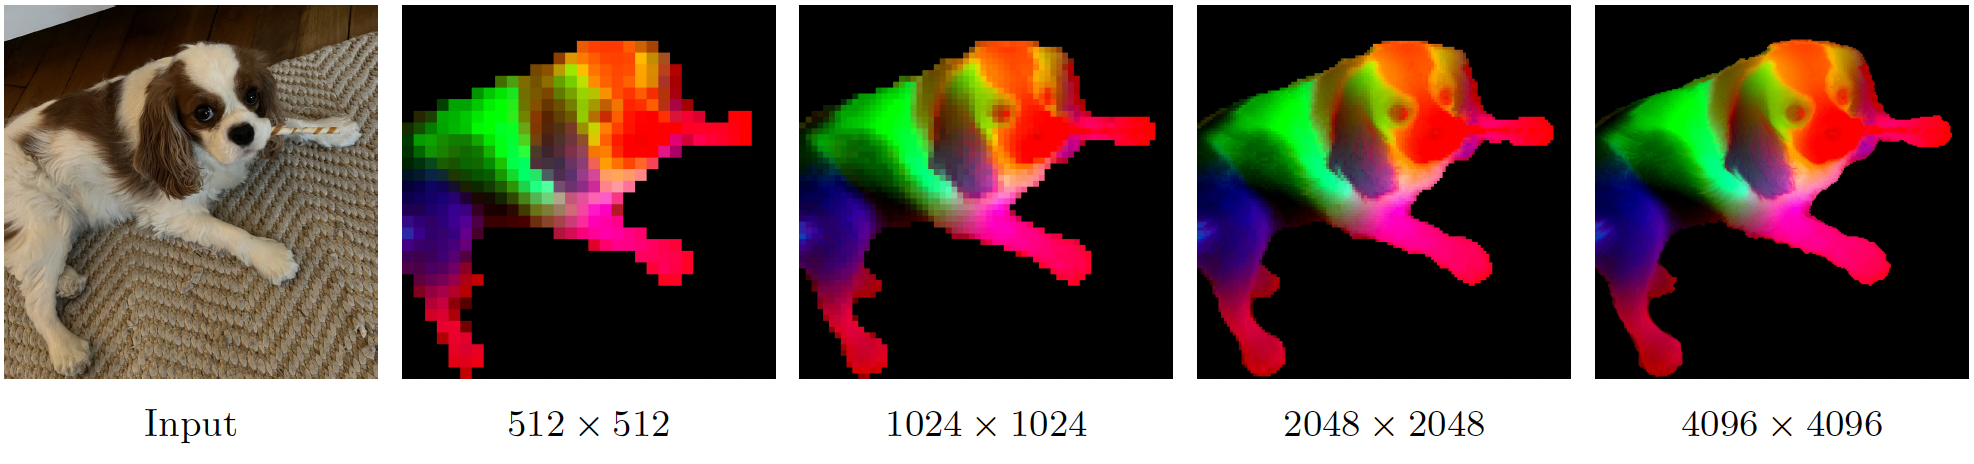
\includegraphics[width=0.8\linewidth]{Presentation2/figures/res-adaptiation.png}
        %\caption{Caption}
        %\label{fig:placeholder}
    \end{figure}
\end{frame}
% ------
\begin{frame}{Evaluation methods}
    Backbone is \textbf{frozen} throughout - only linear/k-NN probes or task decoders are trained
    \vspace{5px}
    \begin{table}
        \centering
        \footnotesize
        \begin{tabular}{>{\raggedright\arraybackslash}p{0.26\linewidth} l >{\raggedright\arraybackslash}p{0.52\linewidth}}
            \toprule
            \textbf{Family} & \textbf{Covered} & \textbf{How DINOv3 evaluates it} \\
            \midrule
            Representation geometry & Partial & PCA→RGB and patch cosine-similarity maps (no UMAP / t-SNE) \\
            Transferability \& robustness & Full & ImageNet-R/Sketch/A, ObjectNet, ImageNet-C, COCO-O, satellite \\
            Downstream performance & Full & Linear probes (cls., seg., depth), k-NN, tracking, task decoders \\
            Representation similarity & None & No CKA / RSA / SVCCA \\
            Diversity / collapse & Partial & Prevented by KoLeo + Sinkhorn; only CLS--patch similarity inspected (no RankMe / eff.\ rank) \\
            \bottomrule
        \end{tabular}
    \end{table}
    \vspace{5px}
    \textbf{2 full, 2 partial, 1 missing} - the evaluation is almost entirely task-based
\end{frame}
% ------
\begin{frame}{Key Results}
    \begin{table}
        \centering
        \footnotesize
        \begin{tabular}{>{\raggedright\arraybackslash}p{0.24\linewidth} >{\raggedright\arraybackslash}p{0.36\linewidth} >{\raggedright\arraybackslash}p{0.28\linewidth}}
            \toprule
            \textbf{Family} & \textbf{Result (frozen 7B)} & \textbf{Interpretation} \\
            \midrule
            Downstream - dense & ADE20k linear 55.9 mIoU (+6.4 vs DINOv2) & Patch features are linearly semantic \\
            Downstream - global & ImageNet linear 88.4 (PE: 89.3) & SSL $\approx$ image--text pre-training \\
            Downstream - systems & COCO 66.1 mAP, ADE20k 63.0 mIoU & One backbone, many tasks \\
            Transfer \& robustness & ObjectNet 79.0 (+12.6 vs DINOv2), best on ImageNet-C & Robust beyond ImageNet \\
            Transfer - domain & Satellite canopy height MAE 2.42 → 2.02 & Recipe is domain-agnostic \\
            Geometry & Clean PCA maps up to 4096 px & Qualitative only \\
            \bottomrule
        \end{tabular}
    \end{table}
    \vspace{5px}
    \textbf{Takeaway:} big win on dense tasks, parity on global tasks - weak on OCR (Logo-2K+ 86.0 vs 93.2 for PE)
\end{frame}
% ------
\begin{frame}{Critique and conclusion}
  \begin{columns}[T]
    \begin{column}{0.32\textwidth}
      \cbox{shown}{Shown}{%
        \begin{itemize}\setlength{\itemsep}{2pt}\setlength{\leftmargini}{8pt}
          \item Dense quality degrades while global keeps improving
          \item Gram: +5.4 mIoU at $-$0.2 IN1k
          \item ViT-H+ $\approx$ 7B teacher
          \item Recipe transfers to satellite
        \end{itemize}}
    \end{column}
    \begin{column}{0.32\textwidth}
      \cbox{hypo}{Hypothesised}{%
        \begin{itemize}\setlength{\itemsep}{2pt}\setlength{\leftmargini}{8pt}
          \item Global loss dominates $\rightarrow$ patches align with CLS
          \item Early checkpoints hold better local structure
          \item SSL keeps scaling like LLMs
          \item Students don't degrade
        \end{itemize}}
    \end{column}
    \begin{column}{0.32\textwidth}
      \cbox{limit}{Limitations}{%
        \begin{itemize}\setlength{\itemsep}{2pt}\setlength{\leftmargini}{8pt}
          \item Private data, curated with DINOv2
          \item Single-run ablations, short schedules
          \item OCR / zero-shot gap
          \item $\approx$2,600\,tCO$_2$e project
        \end{itemize}}
    \end{column}
  \end{columns}
  \vfill
  \begin{center}
    \textbf{Main open question:} are the gains from Gram anchoring,\\
    or from 6$\times$ scale + private data?
  \end{center}
\end{frame}
% ------

% ----------------
% Extra slides
% ----------------
\begin{frame}{Questions}

\end{frame}
%-------
\begin{frame}{Distillation approach}
    
\end{frame}
%-------
\begin{frame}{Evaluation of Dense Features}
    
\end{frame}
%-------
\begin{frame}{Evaluation of Global Image Descriptors}
    
\end{frame}
%-------
\begin{frame}{OOD evaluation - Earth Observation}
    
\end{frame}
%-------
\begin{frame}{Evaluation of Distilled models}
    
\end{frame}
%-------